\section{Design}

To achieve the objectives in \S\ref{sec:bg}, \name{} utilizes a
design/strategy we call ``\emph{decentralized orchestration}'' where instead
of executing workflow orchestration logics entirely with a centralized
orchestrator, a set of ``decentralized orchestrators'' run \emph{in-situ} with
user functions and each performs only the orchestration logic \emph{local to
its subsection} of the workflow.

Efficiently implementing decentralized orchestration while also preserving the
benefits of centralized orchestrators (\S\ref{sec:bg:orchestrator}) requires
\name{} to solve three key problems:

\begin{enumerate}

	\item Given a workflow written in a high-level description language, how
	to divide its orchestration logic such that it can run in a decentralized
	manner in-situ with user functions?

	\item How to efficiently execute orchestration patterns that requires data
	sharing and synchronization across function instances (e.g., fan-in) in a
	decentralized manner?\dhl{Sync with background. explain the challenges of
	fan-in in background.}

	\item How to provide exactly-once execution semantics when the
	orchestration logic is decentralized across function instances that can
	crash and retry at any point mid-execution?\dhl{Sync with background. Need
	to have talked about retries and duplicates already.}

\end{enumerate}

\name{} solves the first challenge \emph{at compile time}, using a frontend
compiler and an intermediate representation (IR). Given a workflow definition
written in a high-level description language, the frontend compiler derives a
directed graph from the high-level description and compile it into the \name{}
IR.


\subsection{High-level Architecture}
\label{sec:architecture}

\begin{figure*}[t]
	\centering
	\begin{subfigure}[t]{0.8\textwidth}
		%        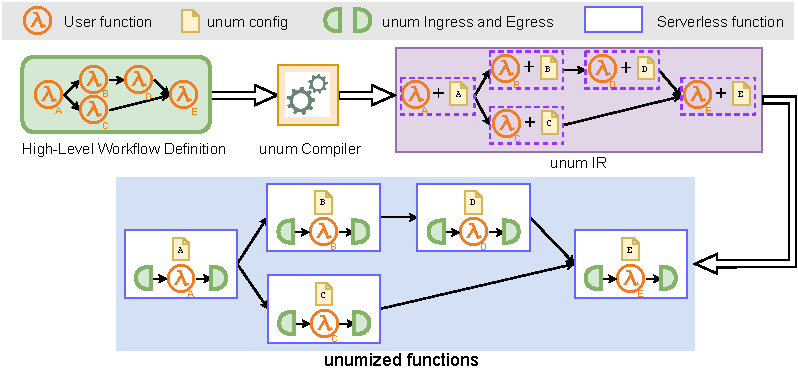
\includegraphics[width=\columnwidth]{figures/unum-arch-compile-time.pdf}
		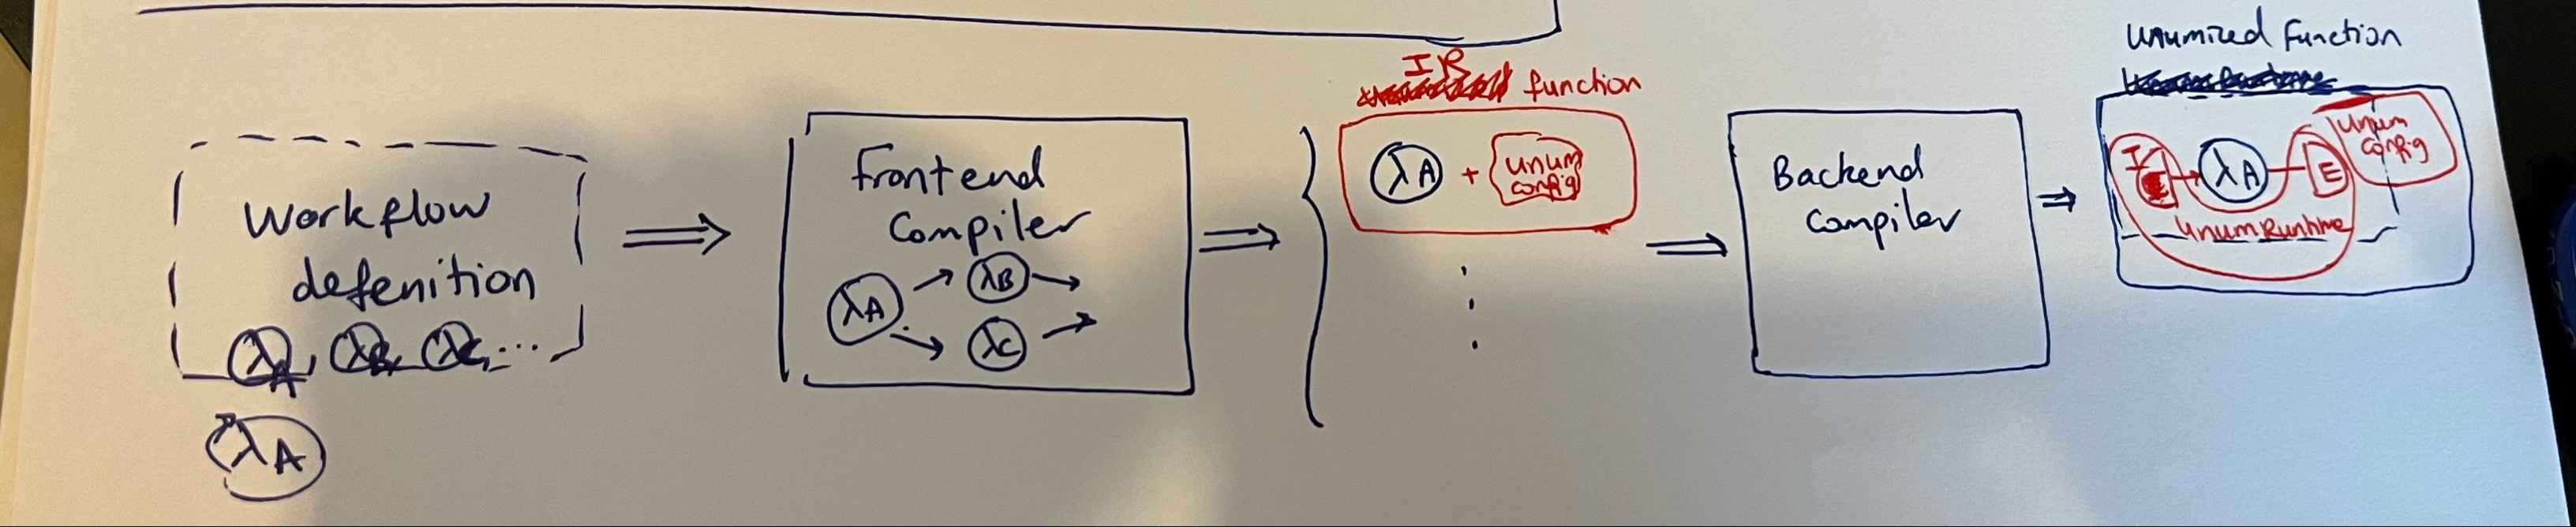
\includegraphics[width=\columnwidth]{figures/architecture.png}
		\caption{Stateful serverless computations form a directed graph. Nodes
			are user defined FaaS functions and ingress and egress ``gadgets'' that perform the necessary data movement, synchronization, and checkpointing between user functions.}
		\label{fig:arch:unum-compile-time}
		% unum injects gadgets to functions at compile time. But more
		% specifically, unum injects an encoding of gadgets at compile time.
		% The encoding expresses control-flow transitions just like what the
		% high-level workflow definition.
	\end{subfigure}
	\begin{subfigure}[b]{\columnwidth}
		\centering
		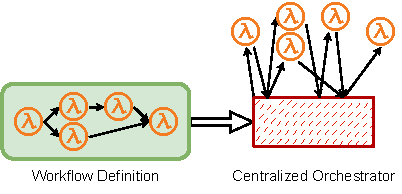
\includegraphics[width=0.8\columnwidth]{figures/unum-arch-centralized.pdf}
		\caption{A typical stateful serverless system drives workflow logic
			using a centralized controller that manages the computation's state-machine.}
		\label{fig:arch:centralized}
	\end{subfigure}
	\hfill
	\begin{subfigure}[b]{\columnwidth}
		\centering
		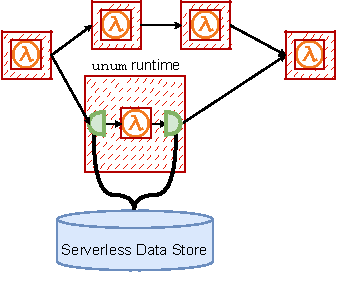
\includegraphics[width=.7\columnwidth]{figures/unum-arch-runtime.pdf}
		\caption{At runtime, all \name{} control logic is decentralized and runs within the Faas 
			functions executed on an unmodified serverless platform. For synchronization and checkpointing, \name{} relies exclusively on a
			standard datastore of choice, such as DynamoDB or Cosmos DB.}
		\label{fig:arch:unum-runtime}
	\end{subfigure}
	\caption{\name{} System Overview. Serverless computations form a directed
		graph that encode sequential and data dependencies between functions. Workflow
		orchestrators drive these graphs by centralizing control flow logic and
		interposing on all communication between functions. \name{},
		instead, decentralizes control flow logic among the functions with
		no need for a separate orchestration system.}
	\label{fig:arch}
\end{figure*}


Similar to other workflow systems~\cite{aws-step-functions, google-workflows,
	google-cloud-composer, gg-atc}, in \name{} users define their workflows using
a high-level description language that (directly or indirectly) expresses the
control-flow in the form of directed graphs  where nodes are serverless
functions and edges are control-flow transitions between functions. \name{'s} modular and extensible design supports integration with all commonly used high-level languages, e.g., Step functions representing workflows as state machines and Google
Workflows, Apache Airflow, Dask, representing workflows as DAGs\footnote{Our current implementation of \name{} is based on Step Functions.}.
%

Different from existing systems where a centralized orchestrator executes
the control-flow graph, \name{} partitions the control flow logic;  embeds the control flow alongside each individual function; and executes the functions in a distributed manner, with no centralized controller or additional services. Figure~\ref{fig:arch:unum-compile-time} shows the steps involved. First, the  \name{} compiler transforms the high-level workflow into a directed graph representation, e.g., converting the Step function state machines to a directed graph. Using this graph, the compiler outputs an platform agnostic intermediate representation (IR) represented as a set of IR functions, i.e, the user functions with the \name{} config embedded into it. the \name{} config includes the configuration on transition from the current function to the next function(s). Thus, instead of having a global view of the control-flow (in an orchestrator), the control-flow is distributed among functions such that each function just need to know where next to send the output. 

Next, the \name{} backend compiler converts the IR functions into \textit{unumized} functions, i.e., platform specific FaaS functions embedded with a \name{} runtime for that platform and the \name{} config. The user then deploys these unumized functions instead of its original functions. Upon execution, based on the \name{} config, the \name{} runtime  transparently, and in a decentralized manner, transitions data accordingly from one function to the next while also providing support for complex patterns such as fan-in. Additionally, the
runtime implements a checkpointing mechanism that ensures exactly-once
semantics (Section \shadi{?}).

This two step process in \name{} with the IR representation, enables portability to different function platforms (e.g., AWS Lambda or Azure Functions), and compatibility to different high-level languages as long as they can be compiled to a directed graph. Our current implementation is based on Step Functions as the API and AWS Lambda as the backend.


In this section, we first describe the transition patterns \name{} supports (Section~\ref{sec:transition-patterns}) and how these are executed in a decentralized manner (Section~\ref{sec:transition-execution}). Then, we describe the how we capture these patterns in our platform-agnostic IR representation (Section~\ref{sec:ir}). Finally, we describe how \name{} provides \shadi{....? describe the last sub sections.}. 



\subsection{\name{'s} transition patterns}
\label{sec:transition-patterns}


We have identified six workflow transition patterns as the main building blocks to build arbitrary workflow compositions. These patterns are simple to use and yet expressive. These patterns include: \shadi{should we add sentence on how fold and for are unique?}

\squishlist
	\item \textit{\textbf{chain:} }
		Chaining is a simple but most fundamental control-flow pattern, e.g.,  a function processing sensor data followed by a function adjusting an	actuator. The \texttt{chain} pattern connects the
		two functions by invoking the target function with the source function's
		result. 

	\item \textit{\textbf{fan out:}} 
	A common pattern to create parallel processing,  e.g.,  an social network application processing a new user post by, in parallel, performing
	 URL shortening
	and resolving users tagged. 
	The fan-out pattern
	launches a vector of functions (branches) with the output of a single
	source function. 
	\item \textit{\textbf{map: }} Map is a simple interface to create parallelism of an identical function, e.g.,  a photo management application performing the same "compression" function on
	each of the images in a unzipped folder.  The map pattern invokes the same
function, once for each element, in a vector of outputs from a single source
function.
	\item \textit{\textbf{fan in:}} is a common pattern to join back multiple parallel functions, e.g., a video encoder that has encoded video chunks each in parallel might want to concatenate all the encoded
	chunks together. The fan-in pattern invokes a single ``sink''
	function with the outputs from a vector of functions (the fan-in branches).
	
	\item \textit{\textbf{fold:}}  \shadiS{is an advanced pattern that is supported by few
		systems~\cite{azure-functions}. Fold sequentially applies the same function on the outputs of a vector of source functions, while aggregating with the intermediate results of running the function so far. An example of fold would be concatenating several video chunks in order: concatenating chunk 1 and 2, then concatenating chunk 3 to chunk [1--2], and so on.
	}
	
	\item \textit{\textbf{branch:}} \shadiS{ is a new pattern supported by \name{} where any  transition pattern can also be conditional, i.e., only execute when the conditions are met. Branch is simple construct with powerful implications, e.g.,  \shadi{@David: example? something in line of "selecting the ML model to run on an image based on the size of the image"}. It also it allows building complex patterns such as ``while'' loops and recursion by using branch as the condition to end the while-loop or recursion. The
	branch pattern selects a next function based on some boolean
	condition. \shadi{why do we call it branch? would conditional work?}
}

\squishend\vspace{-1ex}
	

We found these to be sufficient to express all commonly used orchestrator systems including AWS Step
Functions, \shadi{X, y, and Z} and in many cases they were a super-set of what was provided (e.g., Step functions does not support fold). In addition, we studied several real-world serverless applications and found that the above patterns are sufficient for expressing all.  Below we describe how four representative real-world applications, taken from serverless application repositories and prior research, map to these patterns. These applications represent a diverse set ranging from a simple 2-function IoT pipeline to a complex \shadi{1000s of} functions application.

\noindent\underline{\textit{IoT Pipeline:}} A HVAC control application (in
	AWS serverless repository~\cite{iot-pipeline}) consisting  of a
	two functions connected with a simple chain pattern: a function that aggregates  a time-series data
	on indoor climate readings,  followed by a HVAC system control function that
	adjusts the HVAC settings based on the aggregate climate data.
	
	\noindent \underline{\textit{Text Processing:}} A social network application (adapted from
	the DeathStarBench~\cite{deathstar}) that post-processes a new social network posted by a user.  The workflow consists of 5 functions, following the overall structure of Figure \ref{fig:arch:unum-compile-time}.
	It fans out to two branches that resolves user mentions and shortens URLs
	in parallel. \shadi{what does the chain do?} Lastly, it fans in to a function that saves the post along
	with resolved user mentions and shortened URLs in a NoSQL database.
	
	 \noindent \underline{\textit{MapReduce:}} A word count application (from MapReduce 
	count~\cite{mapreduce}) counting the number of each word in a dataset. The workflow consists of 250 parallel mappers functions each counting words in a subset of the dataset (map) followed by \shadi{one} reducer function aggregating all counts (fan-in).
	
	\noindent\underline{\textit{ExCamera:}} is a novel video encoder ~\cite{excamera} that
	encodes large raw videos with thousands of parallel functions to achieve
	low latency. This application has a complex workflow with use of multiple patterns, as shown in Figure~\ref{fig:excamera} .
%		It breaks a large video into small chunks and runs expensive
%	steps in parallel and fast steps in series. 
	The workflow consists of three
	stages. First, an ``encode'' stage  that chunks the video and runs multiple encoding functions entirely in parallel shown as individual branches in Figure~\ref{fig:excamera}, shown as a map followed by chain pattern. Next, each branch $i$ combines results from the previous branch $(i-1)$ to \shadi{david:?? encode the video based on the previous chunk?}
	. This step involves a series of fan-outs and fan-ins. Finally, all encoded video chunks are concatiated into the a single video stream using a fold and fan-in pattern.
%	
%	 \texttt{ENCODE}, \texttt{ENCODE-GIVEN-STATE} and \texttt{REBASE},
%	where functions interact in complex patterns. The first stage is a
%	\texttt{map} that runs many \texttt{ENCODE} functions entirely in
%	parallel, shown as individual branches in Figure~\ref{fig:excamera}. The second stage forms parallel pipelines following the first
%	stage where the $i^{th}$ \texttt{ENCODE-GIVEN-STATE} branch starts when
%	the $(i)^{th}$ and $(i-1)^{th}$ \texttt{ENCODE} branch complete. The final
%	\texttt{REBASE} runs in series and rebases each chunk on top of the state
%	from the previous chunk (the last fold and fan-in steps).

 \name{'s} set of 6 patterns are sufficient to express a wide range of real-world applications. In the following section, we will describe  how we execute each pattern in a completely decentralized manner.

\begin{figure}[t!]
	\centering
	\scalebox{.9}{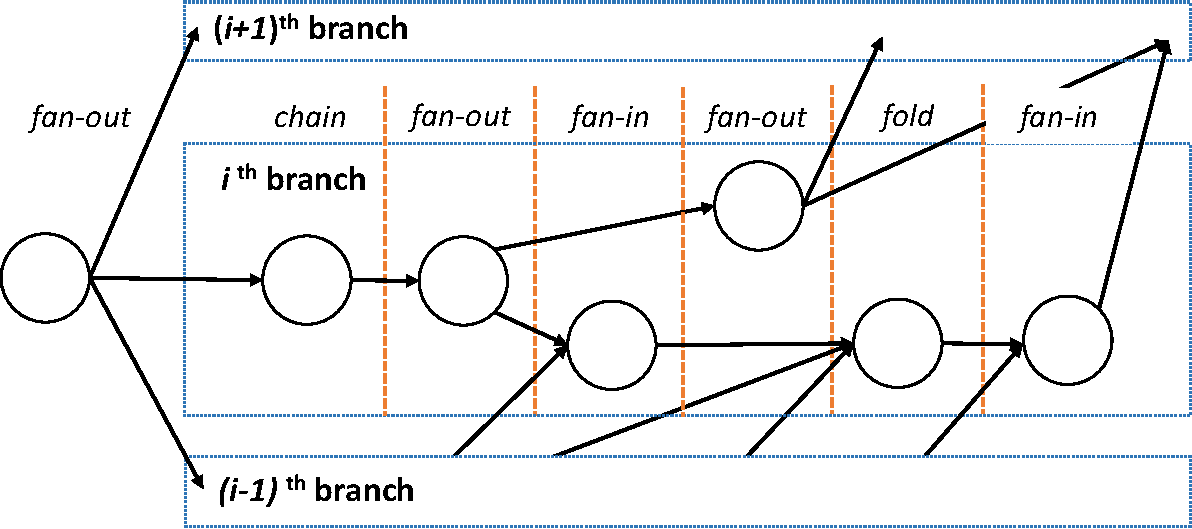
\includegraphics[width=\columnwidth]{figures/excamera.pdf}}
	\caption{ExCamera breakdown of workflow transition patterns. }
	\label{fig:excamera}
\end{figure}


%\name{} supports four general  control-flow/transition patterns: \shadi{do we want to use the name "transition" or "control-flow". Lets be consistent throughout.}
%\begin{itemize}
%	\item \textit{chain} ($f\rightarrow g$): where $g$ is invoked with the output of $f$. Chaining is a simple but most fundamental control-flow pattern, e.g.,  a function processing sensor data followed by another function adjusting an
%	actuator. 
%	\item \textit{map}($f[o_1, ..., o_n]\rightarrow g$): where $g$ is invoked on  \textit{multiple} outputs of $f$. Map is a simple interface to create parallelism but on an identical function, e.g.,  a photo management application performs the same "compression" function on
%	each of the images in a unzipped folder. 
%	\item \textit{fan out} ($f\rightarrow [g_1, ..., g_n]$): where and array of (identical or different) functions, $g_1$ to $g_n$ are invoked in parallel with the output of $f$. Fan-out is a common pattern to create parallel processing,  e.g.,  an social network application performing
%	several independent functions given a new user post, such as URL shortening
%	and resolving other users mentioned in the post. 
%	\item \textit{fan in} ($[f_1, ...f_n] \rightarrow g$): where the output of $n$ (identical or different) parallel functions are aggregated and then $g$ is invoked on the array of \textit{all} outputs. This is a common pattern to join back multiple parallel functions, e.g.,\shadi{??}. 
%\end{itemize}
%
%\name{} applications/workflows are built by using arbitrary composition of  these patterns, e.g., a serverless video encoder that divides a large
%video into chunks(\shadi{?}), encodes each chunk in parallel (map) and concatenates all back
%at the end (fan-in).
%These four patterns  can express a rich variety of workflows
%efficiently, including a superset of workflows expressible in AWS Step
%Functions and all workflows we encountered. In the next section we describe how we execute these pattern with no orchestrator involved.


%
%\subsection{Decentralized execution of transitions}
%\label{sec:transition-execution}
%
%A key challenge in decentralizing control-flow is determining where to store
%control-flow state and how to execute transitions, without a global view of the orchestrator. \name{} decentralized each pattern by logically partitioning the transition into a pair of nodes:  an \textit{egress node(s)} appended to the
%upstream function and a matching \textit{ingress node(s)} prepended to the immediate
%downstream function(s).  Every user function is invoked once with a
%single value by an ingress node and outputs its result to a single egress
%node.  Figure~\ref{fig:transition} demonstrates the ingress/egress nodes added for each pattern. Each ingress/egress node performs a specific logic on the incoming/outgoing data depending on the transition pattern,  as we will discuss further below.  We note that transition patterns only uses the basic serverless abstractions, universally supported by current platforms, and are platform agnostic.
%Specifically, they relies
%on an asynchronous invocation API for FaaS functions and a strongly consistent
%data store that supports conditional writes (for fan-in and exactly-once guarantees only). 
%
%%Logically, each pattern is designed as
%%a pair of nodes: an ingress node and an egress node. The egress node is appended to the
%%upstream function and the matching ingress node is prepended to the immediate
%%downstream function(s).
%%Every user function in
%%\name{} has exactly one input edge coming from an ingress node and one output
%%edge going to an egress node, i.e., the user function is invoked once with a
%%single value by an ingress node and outputs its result to a single egress
%%node. 
%
%%The \name{} backend compiler converts the IR representation of functions  to platform specific \name{} runtimes with pairs of ingress/egress nodes (Figure \shadi{??}). The runtime then, based on the transition patterns embeded in \name{} config file, executes the patterns accordingly in each egress/ingress point. In this section we describe what exact execution logic does each pattern map to at the ingress and egress points. We note that \name{} runtime only uses the basic serverless abstractions, universally supported by current platforms, and are platform agnostic.
%%Specifically, it relies
%%on an asynchronous invocation API for FaaS functions and a strongly consistent
%%data store that supports conditional writes (for fan-in and exactly-once guarantees only). 
%
%\begin{figure}[t!]
%	\centering
%	\scalebox{.7}{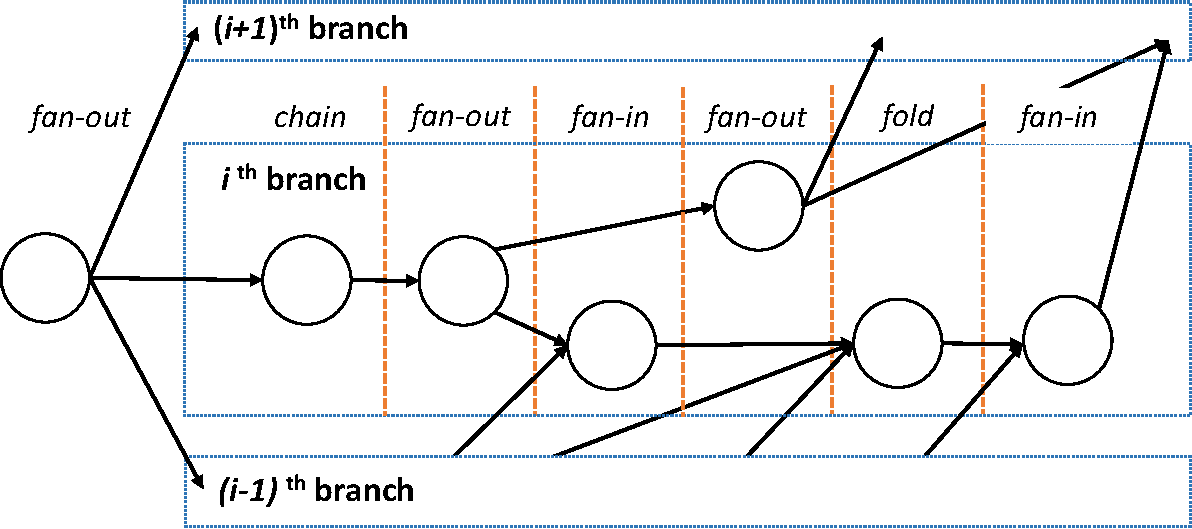
\includegraphics[width=\columnwidth]{figures/excamera.pdf}}
%	\caption{TODO}
%	\label{fig:excamera}
%\end{figure}
%
%\noindent\textbf{Chain:}
%The chain pattern invokes a single target function with the result of a source function.
%As shown in Figure~\ref{fig:transition}, chaining consists of one egress node 
%appended to the source function and one ingress is prepended to the target.
%At runtime, the egress node gets the output of the source user function
%and uses the platform's asynchronous function invocation API to call the
%target function directly from the source. The ingress on the target reads the
%data sent from source and passes it to the target user function. Depending on
%the platform's implementation of asynchronous invoke API, the ingress might
%read the input data from a data store or the received HTTP message.
%
%
%\noindent\textbf{Fan-out:}
%The fan-out processes the output of a function  in parallel, by 
%invoking vector of functions (branches) each with the output of the same
%source function. The fan-out pattern consists of one egress node and many ingress
%nodes (one per branch). Similar to chaining, the egress node runs with the
%source function and it uses the asynchronous invocation API to invoke each
%branch where each ingress node 
%reads the input data sent from the source and passes it to its user function.
%
%
%\noindent \textbf{Map:}
%The \texttt{map} gadget invokes the same
%function once for each element in a vector of outputs from the source
%function. The algorithm and placement of \texttt{map} ingress and egress nodes
%are identical to \texttt{fanOut}. \dhl{TODO: talk about the dynamic aspect of Map}
%\shadi{Map seems very empty. why do we have it separated? any details and challenges to add here? }
%
%
%
%
%\noindent\textbf{Fan-in:} The \texttt{fanIn} pattern takes the outputs from a vector of
%functions (the fan-in branches) and invokes a single ``sink'' function. As shown in Figure~\ref{fig:transition}, fan-in consists of one ingress prepended to the sink function and several egress nodes, each
%appended to a fan-in branch. Fan-in has an important requirement--the sink function should be called \textit{once} and only when \textit{all} fan-in branches have completed. At the same time, \name{} aims to avoid idle-billing and therefore extra billing (Section \shadi{??}). Thus, the fan-in pattern should be ``wait-free'' on both sides: a) the upstream functions should terminate after completion and not wait for each other, and b) the sink function should not  spin up ahead of time idly waiting for upstream functions to finish.
%
%% TBD
%%
%% The \texttt{fanIn} gadget gadget ensures that the control-flow transition is
%% \emph{wait-free} and that the sink function is invoked only once.
%% Specifically, its semantics is that the sink function is invoked only once
%% when all upstream functions in the vector have completed.
%
%% To realize the semantics, the \texttt{fanIn} gadget has to solve several
%% challenges. Access to branches data. wait-free. and synchronize.
%
%%The \texttt{fanIn} gadget ensures that the control-flow transition is
%%\emph{wait-free}. That is the sink function is invoked only when all upstream
%%functions in the vector have completed so that the sink function does have to
%%be spun up ahead of time and waste CPU cycles (and therefore extra billing)
%%idly waiting for upstream functions to finish. Moreover, the upstream
%%functions in \texttt{fanIn} simply terminates when done and do not wait for
%%each other either.
%
%To achieve this, \name{} uses an intermediary data store (as shown in Figure \shadi{??}) to log the output of upstream functions and signal the completion to the sink. In this design, each egress  node simply
%writes its output and terminates the function (avoiding idle-billing on the upstream functions), with the exception of the ``last'' egress node which first invokes the sink function. \name{} synchronizes among the upstream functions to identify the ``last'' function using an
%atomic read-after-write over a single object. Every upstream function \shadi{....? give a high-level idea. what is the process here, a few senteces in the data-store independent manner!}.  This ensures when the sink function is
%invoked, it is invoked only once.  Specific implementation depends
%on the data store as we discuss the details in \S\ref{sec:impl}.  Given that the data store is shared among all upstream functions, any egress node can see if another egress node has completed and any egress can invoke the sink function. 
%
%The ``last'' egress invokes the sink function with a vector of pointers
%to each upstream function's stored output. The pointers are the in same order
%as the vector of upstream function names.\shadi{does this point regarding the naming matter? if so, add some details. If not, maybe remove?} The ingress on the sink function
%dereferences each point by reading from the data store and passes a vector of
%output values to its user function.
%
%
%We have implemented \name{} with both Dynamo DB and S3. However, \name{} can be integrated with any data-store as long is it provides strong consistency with conditional writes. Strongly consistent is required to prevent the
%scenarios where all egress nodes have written outputs but none of them sees that all
%have completed, which will result in the sink function never being invoked. \shadi{wouldn't eventual be enough? the sink will eventually be invoked}
%\shadi{give insight why you need conditional writes. this comes out of the blue}. 
%\dhl{?TODO: Say more about synchronization? That it needs to be idempotent
%	because functions can crash and be retried.}
%
%
%%To achieve this, the \texttt{fanIn} egress always writes the output of its
%%user function to a data store. This serves two purposes: (1). it allows any of
%%the upstream functions to access the output of other upstream functions (2).
%%it signals the completion of a function. This way, each egress can simply
%%writes its output and terminate. 
%%
%%Other egress nodes can still access completed
%%egress' data after they terminate. Any one of the egress can invoke the sink
%%function. And any one of the egress can see if other egress has completed or
%%not. \dhl{definitely needs better phrasing but hopeful the point makes sense}
%
%
%
%
%
%
%\dhl{?TODO: Fan-in is a critical control-flow pattern to support and distinguishes \name{}
%	from ad-hoc trigger-based composition.  Do we want to constrast here? and what
%	should we say? Different from ad-hoc compositions: 1. use of data store 2.
%	Control flow logic not only on the caller but also on the callee 3. standard,
%	off-the-shelf primitives that's not application specific that developers build
%	from scratch.}
%
%\dhl{?TODO: Fan-in expresses data dependencies. More flexible/expressive than
%	Step Functions because SF only supports dependencies within a state. unum
%	fan-in can specify any function in the workflow.}
%
%
%
%
%
%
%
%
%
%
%
%
%
%\shadi{:::::::::left over comments. not sure if they need to be addressed?}
%
%
%
%%
%%\amit{TODO: I feel like there is a bunch of complexity, particularly with
%%	fan-in, do with assigning indexes to branches, etc, that is part of the
%%	platform-agnostic design of unum, so should be here. But I don't recall the
%%	specifics. Are there also similar things for the other gadgets?}
%%\dhl{I'm not sure what you mean by "similar things". But the branch indexes
%%	are assigned by the fan-\emph{out} node. The purpose is to give each node in
%%	the graph a unique name. I really don't think we should discuss the naming
%%	aspect in this section. I think this structure of writing the design works
%%	very well if we keep the gadgets to be general algorithms for control-flow
%%	patterns that are designed against an abstract serverless machine. We can talk
%%	about what we require from the serverless abstraction, but we shouldn't talk
%%	about the naming scheme. The gadget just cares that each function has a name,
%%	that you can identify them. It does not care how. Then in the IR section, we
%%	can talk about how the IR actually encodes the gadgets, and that's where we
%%	can explain that (1). we need each function to have a unique name for fan-in
%%	to work because we need to clearly identify which node's result to fan-in
%%	from, and we can have multiple instances of the same function in the graph
%%	because of fan-in and map. (2). our naming scheme is to assign an integer,
%%	starting with 0 and incrementing monotonically by 1, to each branch. And
%%	that's it. That's all the information we need at the IR level. And finally in
%%	the runtime section, we show the input payload which has a field for the
%%	branch index, and that's how we actually implement this piece of information.
%%	And we explain that the fan-out node adds this field to the payload when
%%	invoking each branch. It's like the storage layers where each layer adds a bit
%%	more information to enable specific additional functionalities.}
%
%
%
%
%% chain = invoke, fan-out = a bunch of invoke, one for each continuation;
%% Additionally, in the case of Map, one invoke for each element of the array
%% (output of the user function).  fan-in .... well.... let's see. The semantics
%% is: invoke the fan-in function once when all of its inputs are ready. In
%% practice, it is each branch synchronize over the data store to see if all
%% branches have completed. The last branch to complete calls invoke on the fan-in
%% function, and pass it pointers to all branches results/checkpoints in the data
%% store. The fan-in function first reads the branches' results, in order, via the
%% pointers, then pass them as input to the user code.
%
%\dhl{"strongly consistent data store with conditional writes". Is this going
%	to raise eyebrows when we later mention S3? Because technically, S3 does not
%	have a conditional write API. We implement it with its object versions
%	feature, which has to be turned on when creating the bucket. Maybe better to
%	call it something else.}
%
%% \dhl{I'm not sure it makes sense to treate fan-in specially on the directed
%	% graph level. In the previous version, the ingress gadget node on the fan-in
%	% doesn't really perform any \emph{control-flow logic}. It just reads the input
%	% data. And this is the same behavior across all gadgets. The ingress just read
%	% data, whether from a HTTP packet or from DynamoDB. You can pass a vector of
%	% pointers via a chain gadget and the ingress will do the same thing. But I
%	% guess more importantly, the ingress is simply and uniform enough that treating
%	% fan-in specially in our explanation doesn't add much value.}
%
%\dhl{From previous version: "At compile-time, \name{} injects these gadgets
%	into the nearest function and executes them in the \name{} runtime that wraps
%	the function. Thus there is no system overhead for running the gadgets---they
%	are, effectively, embedded in the functions themselves."The last sentence is
%	unclear to me. Running gadgets incur latency and additional Lambda billing.}
%
%%%%%%%%%%%%%%%%%%%
\subsection{\name{} Intermediate Representation}\label{sec:ir}

\begin{figure*}[t!]
	\centering
	\begin{subfigure}[t]{\columnwidth}
		\centering
		\begin{minted}[
			frame=single,
			fontsize=\scriptsize
			]{json}
{
	"Name": "F",
	"Next": {
		"Name": "G",
		"InputType": "Scalar",
		"Conditional": true,
	}
}
		\end{minted}
		\caption{\texttt{chain} pattern that invokes function \texttt{G} with
			\texttt{F}'s result}
		\label{fig:gadget-examples-chain}
	\end{subfigure}
	\begin{subfigure}[t]{\columnwidth}
		\centering
		\begin{minted}[
			frame=single,
			fontsize=\scriptsize
			]{json}
{
	"Name": "M",
	"Next": {
		"Name": "N",
		"InputType": "Map"
	}
}
		\end{minted}
		\caption{\texttt{map} pattern that invokes a parallel instance of
			\texttt{N} for each element of the vector output of \texttt{M}}
		\label{fig:gadget-examples-map}
	\end{subfigure}
	\hfill
	\begin{subfigure}[t]{\columnwidth}
		\centering
		\begin{minted}[
			frame=single,
			fontsize=\scriptsize
			]{json}
{
	"Name": "G",
	"Next": [
	{
		"Name": "H",
		"InputType": "Scalar"
	},
	{
		"Name": "M",
		"InputType": "Scalar"
	}
	]
}
		\end{minted}
		\caption{\texttt{fan-out} pattern that invokes function \texttt{H} and
			\texttt{M} with the result of \texttt{G}}
		\label{fig:gadget-examples-fanout}
	\end{subfigure}
	\begin{subfigure}[t]{\columnwidth}
		\centering
		\begin{minted}[
			frame=single,
			fontsize=\scriptsize
			]{json}
{
	"Name": "N",
	"Next": {
		"Name": "S",
		"InputType": {
			"Fan-in": {
				"Values": [
				"N-unumIndex-*"
				]
			}
		}
	}
}
		\end{minted}
		\caption{\texttt{fan-in} pattern that invokes function \texttt{S} with
			the result of all \texttt{N} instances of a \texttt{map}.}
		\label{fig:gadget-examples-fanin}
	\end{subfigure}

	\begin{subfigure}[t]{\columnwidth}
		\centering
		\begin{minted}[
			frame=single,
			fontsize=\scriptsize
			]{json}
{
	"Name": "F",
	"Next": [
	{
		"Name": "G",
		"InputType": "Scalar",
		"Conditional": "$ret < 0"
	},
	{
		"Name": "H",
		"InputType": "Scalar",
		"Conditional": "$ret >= 0"
	}
	]
}
		\end{minted}
		\caption{\texttt{F} branches on the user function's result by
		combining \texttt{fan-out} with \texttt{Conditional}}
		\label{fig:gadget-examples-branch}
	\end{subfigure}

	\begin{subfigure}[t]{\columnwidth}
		\centering
		\begin{minted}[
			frame=single,
			fontsize=\scriptsize
			]{json}
{
    "Name": "F",
    "Next": {
        "Name": "F",
        "InputType": {
            "Fan-in": {
                "Values": [
                    "F-unumIndex-$0",
                    "G-unumIndex-($0+1)"
                ]
            }
        },
        "Conditional": "$0 < $size-1"
    },
    "Next Payload Modifiers": ["$0=$0+1"]
}
		\end{minted}
		\caption{\texttt{fold} pattern that folds \texttt{F} on the output of
		a vector of \texttt{G} functions}
		\label{fig:gadget-examples-fold}
	\end{subfigure}

	\caption{The \name{} IR representation of common transition patterns.}
	\label{fig:ir-examples}
\end{figure*}
\shadi{the paper suddenly jumps into details of the IR. we still haven't established how we are doing the decentralized orchestration, which is much more important than the IR syntax. I would first discuss the deorc, how the patterns are supported and then the IR.} \shadi{I like the high-level architecture, but this section forward has too much details too soon. We should have a discussion on the flow of this and the next section.}

Before executing serverless workflows in a decentralized manner, a workflow
definition first needs to be partitioned such that each function performs only
the orchestration logic local to its subsection of the workflow. The \name{}
intermediate representation solves this problem with a naming scheme that
uniquely identifies each function instance in the workflow and a configuration
language in JSON that encodes workflow transitions.\shadi{this is another instance of jumping to details without the big picture. you suddenly talk about naming structure and json without giving the details of what this config contains (the following sentences)} Specifically, each
function is assigned a configuration that contains: i. \textit{which}
function(s) to run next, ii. \textit{when} the next function(s) should run,
iii. \textit{what} input should the next function(s) run with.

Note that the IR configuration is platform-agnostic. In particular, it does
not specify how to launch the next function(s), and how to send input data to
the next function(s). These details are left to the \name{} runtime library
(\deorc{}) that can target specific platforms (for example, the \deorc{} for
AWS runs functions as lambdas and uses the Lambda asychronous invocation API
to launch functions). Thus, workflows are portable across platforms by simply
changing the \deorc{} library.

The \name{} frontend compiler can generate IR from workflow definitions
written in high-level description languages (e.g., AWS Step Functions), but
developers can also write IR configurations directly, with just a few lines of
JSON. In particular, The \name{} IR uses a top-level \texttt{Name} field to
identify the source function that the configuration is co-located with, a
\texttt{Next} field to list the workflow transitions, and under which a
\texttt{Name}, \texttt{Conditional}, and \texttt{InputType} fields that
identify which function to run, when and with what input.
Figure~\ref{fig:ir-examples} shows examples on how to express common
orchestration patterns such as branching, chaining, map, fan-out, fan-in and
fold: 

\dhl{Sync with background. should have at least mentioned some of those patterns in
the background.}

\shadi{you suddenly jump into these patterns. why these? where did they come from? this might be the right place to have the apps discussed.}

\paragraph{chain}

%Chaining is a simple but common orchestration pattern. For example, an
%application might include a function (the source) that processes input data
%from a sensor followed by another function (the target) that adjusts an
%actuator based on the processed input. The \texttt{chain} pattern connects the
%two functions by invoking the target function with the source function's
%result.

Figure~\ref{fig:gadget-examples-chain} expresses a chain with a \texttt{Next}
field that contains a single JSON object whose \texttt{InputType} is
\texttt{Scalar}. \texttt{Scalar} means that the target function (i.e.,
\texttt{G}) should receive as input the source function's (i.e., \texttt{F}'s)
output as a singular entity. The \texttt{Conditional: true} means that this
transition should always take place whenever \texttt{F} produces a result.
\texttt{Conditional} is assumed to be \texttt{true} when not specified.

\paragraph{fan-out}

%Another common pattern processes the output of a function in different ways in
%parallel. For example, an social network application might perform several
%independent functions given a new user post, such as URL shortening and
%resolving other users mentioned in the post. The \texttt{fan-out} pattern
%launches a vector of functions (branches) each with the output of the same
%source function.

Figure~\ref{fig:gadget-examples-fanout} expresses a fan-out with an array in
the \texttt{Next} field. Each item of the array identifies a different target
function that should should run in parallel. The \texttt{InputType} field is
\texttt{Scalar} for both branches because both should receive as input the
source function's (i.e., \texttt{F}'s) output as a singular entity.

\paragraph{map}

%An application may also perform the same function on multiple outputs of a
%source function. For example, a photo management application might unpack an
%archive of high-resolution images in one function and perform compression on
%each of the resulting images. The \texttt{map} pattern invokes the same
%function once for each element in a vector of outputs from the source
%function.

Figure~\ref{fig:gadget-examples-map} expresses a \texttt{map} with a
\texttt{Next} field that contains a single JSON object whose
\texttt{InputType} is \texttt{Map}, which indicates that the source function's
(i.e., \texttt{F}'s) output should be treated as an array and for each
element, a target function (i.e., \texttt{G}) should launch with that element
as the input.

\paragraph{fan-in}

%After processing data with many parallel branches, applications commonly want
%to aggregate results. For example, a video encoder might divide a large video
%into chunks, encode each in parallel and then concatenant all the encoded
%chunks together. The \texttt{fan-in} pattern invokes a single ``sink''
%function with the outputs from a vector of functions (the fan-in branches).

Figure~\ref{fig:gadget-examples-fanin} expresses a \texttt{fan-in} with a
\texttt{Next} field that contains a single JSON object whose
\texttt{InputType} is \texttt{Fan-in} under which a \texttt{Values} fields
specifies an ordered list with names of functions whose results should be the
target function's (i.e., \texttt{S}'s)input.

Different from \texttt{Scalar} and \texttt{Map} where the target function only
depends on the source function's output, \texttt{Fan-in} expresses data
dependencies across functions which is difficult to implement efficiently. We
discuss how we support \texttt{fan-in} in \S\ref{sec:runtime}.

\paragraph{branch}

%An application may decide to take a different branch of the workflow graph
%based on runtime behavior (e.g., the output of a function). The
%\texttt{branch} pattern selects a next function based on some boolean
%condition.

Figure~\ref{fig:gadget-examples-branch} expresses a \texttt{branch} with an
array in the \texttt{Next} field where each branch has a \texttt{Conditional}.
Notice that \texttt{branch} is expressed similarly as \texttt{fan-out}
combined with the \texttt{Conditional} field. This example demonstrates the
flexibility and expressiveness of \name{} IR's building blocks which
developers can compose to express additional patterns.

\paragraph{fold}

In functional programming, \texttt{fold} is higher-level function that takes
another functions and applies it to an vector of values. In serverless
workflow, \texttt{fold} is an advanced pattern that is supported by few
systems~\cite{azure-functions}. Although \name{} is built on a simpler
abstraction without adding new components, we support folding a function on
the output of a vector of functions.

Figure~\ref{fig:gadget-examples-fold} expresses a \texttt{fold} that folds the
function \texttt{F} on a vector of \texttt{G} instances result, using a
combination of \texttt{Fan-in}, \texttt{Conditional} and \texttt{Next Payload
Modifiers}. On a high-level, \texttt{F} recursively calls itself, passing the
previous iteration's output (\texttt{F-unumIndex-\$0}) and the next \texttt{G}
instance's result (\texttt{F-unumIndex-(\$0+1)}), until it reaches the last
\texttt{G} instance in the vector ((\texttt{Conditional: "\$0<\$size-1"})). On
each iteration, \texttt{F} increments its index by 1 (\texttt{"\$0=\$0+1"}).
We explain the details on \name{} IR's naming scheme and the use of index and
runtime variables (e.g., \texttt{\$0}) in the next section.


\subsubsection{Naming and Dynamic Runtime Behavior}\label{sec:ir:naming}

A key design challenge of the \name{} IR is to support dynamic runtime
behavior with statically generated configurations.

For instance, in a workflow that consists of a \texttt{map} followed by a
\texttt{fan-in}, \texttt{map} creates multiple parallel instances of the same
function, but the number of instances depends on the output data and cannot be
known at compile-time. \name{} needs to uniquely identify each function
instance so that \texttt{fan-in} can execute correctly (e.g., not miss an
instance or counting the same instance twice).

To solve this problem, \name{} defines a naming scheme for runtime instances
and exposes a set of APIs to interact with names. First,
\name{} requires each user function to have a user-defined name (in the
top-level \texttt{Name} field). This is also a common requirement for existing
serverless systems when developers deploy their functions. Next, each branch
in a \texttt{map} and \texttt{fan-out} pattern is assigned an integer index,
starting from zero, and the $i^th$ branch is named
\texttt{<FunctionName>-unumIndex-\emph{i}}. For nested fan-outs, the indexes
are delimited with periods. For example,
\texttt{<FunctionName>-unumIndex-\emph{i.j}} identifies the $i^{th}$ branch in
the outer loop and $j^{th}$ in the inner loop.

To identify all branches, the \name{}~IR supports glob patterns, such as
\texttt{*}, when specifying runtime instances' names.
Figure~\ref{fig:gadget-examples-fanin} shows a \texttt{fan-in} example that
invokes \texttt{S} with the outputs from all instances of \texttt{N}.

\name{} IR provides a set of runtime variables and APIs that enables
additional dynamic behavior. For example, \texttt{\$0} refers to the
inner-most index of the function instance which can be used in the
\texttt{Values} field for fan-in when input depends on specific instances
instead of all instances. The \texttt{Next Payload Modifiers} field allows
expressions that can modify the runtime variables (e.g., \texttt{\$0=\$0+1}),
which can implement fold or for loops when combined with a termination
condition in \texttt{Conditional}.


\name{} IR also provides other APIs that interacts with runtime data, such as
\texttt{\$ret} that refers to the function's output, and \texttt{\$size} that
refers to the number of parallel branches in a \texttt{map}.







Efficiently executing workflows in a
decentralized manner requires solving three challenges.

Most workflow language directly or indirectly express a directed graph
(\S\ref{sec:bg}.\dhl{Sync with Background. make sure to explain this already}

Instead of a centralized orchestrator executing workflows, \name{}



\subsection{\name{} Runtime}

\begin{figure}[]
    \begin{minted}[
    frame=single,
    fontsize=\scriptsize
  ]{json}
{
    "Data": {
        "Source": "http | dynamodb | s3 | ...",
        "Value": "<object> | [<pointers>]"
    },
    "Session": "uuid",
    "Fan-out": {
        "Index": "int",
        "Size": "int",
        "OuterLoop": {
            "Index": "int",
            "Size": "int"
        }
    }
}
    \end{minted}
    \caption{\name{} runtime input payload schema}
    \label{fig:input-format}
\end{figure}

The primary purpose of the \name{} runtime is to implement the transition with
platform-specific APIs and manage runtime metadata that is required by the
\name{} IR naming scheme and programmable constructs. We design the runtime to
wrap user code and transparently interpose on its entry and exit so that we do
not change how developers write application code.

 \name{} requires a specific input payload schema in JSON
(Figure~\ref{fig:input-format}). When a function is invoked, the input data is
first received by the runtime ingress. The ingress uses the \texttt{Data}
field to read the user function's input data. If the \texttt{Source} is
\texttt{http}, the input data is directly embedded in the \texttt{Value}
field. Otherwise, \name{} uses the pointers in \texttt{Value} to read the
input data from the intermediary data store.

After user function returns, the egress runtime gets its output and checks the
IR configuration to see if there is a transition to execute. If no, it simply
terminates. If yes, it checks if the \texttt{Conditional} evaluates to true
and then executes the transition's egress.

\name{} keeps all runtime metadata in the input payload such that the
functions remain stateless and do not need to persist data via a data store
across invocations. \name{} uses the \texttt{Fan-out} field to store branch
indexes. The \texttt{Fan-out} field contains a recursive \texttt{OuterLoop}
field that \name{} uses to support nest fan-outs.

The runtime additionally uses a \texttt{Session} field to support concurrent
invocations of the same workflow. The \texttt{Session} field is a UUID string
that is unique to a workflow invocation and shared by all constituent function
instances in the invocation. Function checkpoint names are prefixed by the
\texttt{Session} string so that concurrently invocations do not overwrite each
other's data.

The \name{} runtime also implements exactly-once semantics with a
checkpointing mechanism which we discuss in the next section.


\section{Execution Guarantees}

An important characteristic of any workflow system 
is (a) how it deals with  a transient failure in a constituent step, and 
(b) what guarantees it makes in the presence of such faults.
 
Most workflow systems use checkpointing to limit the scope of re-execution after faults. 
In \name{}, each function is checkpointed to storage after it completes. In particular, if a
workflow experiences crashes mid-execution, \name{} does not retry from the beginning but
from the node of failure only.

\name{} guarantees \textbf{exactly-once execution}, meaning that each step of the 
workflow appears to execute exactly once. Even though FaaS engines already support automatic retries for functions,
they only guarantee at-least-once execution. Strengthening this guarantee requires dealing with the following subtleties:
\begin{itemize}
\item Function executions are not always deterministic, each re-execution may produce a different result.
\item The FaaS engine may detect failures incorrectly, thus multiple executions of a function can be in progress simultaneously.
\end{itemize}

Fortunately, we found a way to handle these challenges by taking advantage of conditional store operations 
supported by strongly consistent data stores. 
Specifically, \name{} guarantees that even if there are
multiple function execution instances, concurrent or not, only one instance's result is
taken as the final result and propagates to the downstream ingress node(s).
Other instances simply discard their results and terminate. 

\paragraph{Checkpoints and Synchronization.}
%\name{} uses a similar checkpointing technique across all transition patterns. 
After user code completes, the \name{} egress gadget immediately writes a checkpoint file that contains the user code
results to the intermediary data store. The checkpoint is uniquely named with
the instance's name (i.e., the name according the
\name{}~IR's naming scheme (\S\ref{sec:ir:naming}), prefixed by the workflow
invocation's unique session ID) such that the existence of a checkpoint
implies the corresponding function has successfully completed its user
function. The create operation is a conditional write and only succeeds when
the file does not already exist. If there are concurrent duplicate instances,
only one of them will create the checkpoint. The others will receive an error
from the write operation and \name{} runtime will simply terminate the
instance. The instance that successfully creates a checkpoint will proceeds to
executing its egress node and propagate its result to downstream functions.

For nonconcurrent duplicates (e.g., retries), \name{} checks if a checkpoint
exists \emph{before} running its user code. If a checkpoint does not exist,
\name{} goes ahead and runs the user code. Otherwise, \name{} reads the data
from the checkpoint and use that as final result without running user code
again. Then \name{} will run the ingress node to invoke the downstream function.
This is necessary because the duplicate might be a retry whose prior execution
crashed after checkpointing but before running the downstream ingress node. \name{} can
tolerate running a ingress/egress node more than once because of the same protection
against duplicates.

\paragraph{External Side Effects.}
In the applications targeted by \name{}, there is no need for functions to directly call external storage services. 
Rather, all functions are "side-effect-free": their only effect is to provide a result.
Therefore, the "exactly-one-result" guarantee of the \name{} runtime is in fact synonymous with exactly-once execution.

Although it is not currently required by any of our applications, it is conceivable to extend \name{} in the future to support
workflows whose functions have additional side effects. For example, a store interposition mechanism (such as used in Beldi \cite{beldi}) could 
be added to support functions that require more complex storage interactions than obtaining an input and producing a result.


\amit{TODO: Are there special considerations for exactly-once
	semantics? i.e. is checkpointing different than it is in chaining?}
\dhl{No. In fact checkpoint works independently from the control-flow
	patterns. The algorithm for exactly-once semantics is the same across all
	gadgets.
	
	Now specifically for fan-out it works like this: the fan-out initiator node
	will checkpoint right after user code returns which saves the data that is
	about to be fanned out. After checkpointing completes, the fan-out initiator
	node invokes the branches. If it crashes at any point during the series of
	invocations, unum retries the fan-out initiator lambda. The unum runtime on
	the lambda will see that a checkpoint with its name already exists, and
	therefore skips running the user function. But it will not skip retrying the
	fan-out, and it restarts the fan-out \emph{from the beginning}, which will
	result in duplicate instances for some or even all of the branches. But that
	is OK. Because the unum runtime protects against duplicates and still ensures
	exactly-once semantics. If the duplicates are concurrent (i.e., the original
	branch instances are still running), we protects that with a conditional write
	when checkpointing the results so only one instance of the duplicates will
	win. If the duplicates are nonconcurrent (i.e., the original branch instances
	already completed), the duplicates will skip running the user functions
	altogether.
	
	The fan-out initiator will keep retrying until a full fan-out is performed to
	make sure at-least-once invocation.
	
	% (explaining this makes me appreciate the consistency papers even more, 'cuz
	% this stuff is hard to explain.)
	
	So the patterns do not change the algorithms with which we provide exactly
	once. They work independently from each other. The only real gotcha we need to
	be careful with in \emph{implementing} exactly-once is nonidempotent
	operations, as pointed out by you. Specifically, the synchronizations across
	branches have to be idempotent. The purpose is prevent pre-mature fan-in.
	
}